% siminos/blog/Mathematica.tex
% $Author$ $Date$
%    this is master file: siminos/cgang/2modes.tex
%    \section{{\twoMode} daily blog}
%    \label{chap:2modes}


\subsection{Blogging simulations progress}
\label{s:MathematicaBlog}

\begin{description}
\item[2012-06-11 Predrag]
started a new blog, for Chaos Gang {\twoMode} simulations.

\texttt{siminos/blog/Mathematica.tex}

\item[2012-04-25 Evangelos]
Wrote an interactive Mathematica program, with sliders for parameters:

\texttt{siminos/cgang/Evangelos/dangelmayr\_so2\_int.nb}

\item[2012-04-25 Evangelos]
Dangelmayr system with Predrag's modification
becomes very interesting. It's very easy to find chaotic behavior and in many
cases it seems that asymptotic dynamics are $3$-dimensional.
After spending some time playing with parameters, I've found some
for which it seems we have chaos (at least we can see some stretching
and folding) while a $2$-dimensional description might be possible
(a simple $2$-d branched manifold).
The parameters are
\[
 \mu_1 = -0.337,\, \mu_2 = 0.27,\, c_1 = 1,\, c_2 = -1,\, a_1 = -1.5,\,
 a_2 = -6.19,\, b_1 = 1.583,\,  b_2 = -0.115,\, e_2 = 1.211\,.
\]
I would suggest playing with \texttt{siminos/cgang/Evangelos/dangelmayr\_so2\_int.nb}
to locate \emph{nearby} parameters which you think will give more interesting
results or just explore the system with the parameters given here.

%%%%%%%%%%%%%%%%%%%%%%%%%%%%%%%%%%%%%%%%%%%%%%%%%%%%%%%%%%%%%%%%%%%%%%%%%%%%%%%%%%%%
 \begin{figure}
%% ES created with siminos/cgang/Evangelos/dangelmayr_so2_plot.nb
\centering
 (a) 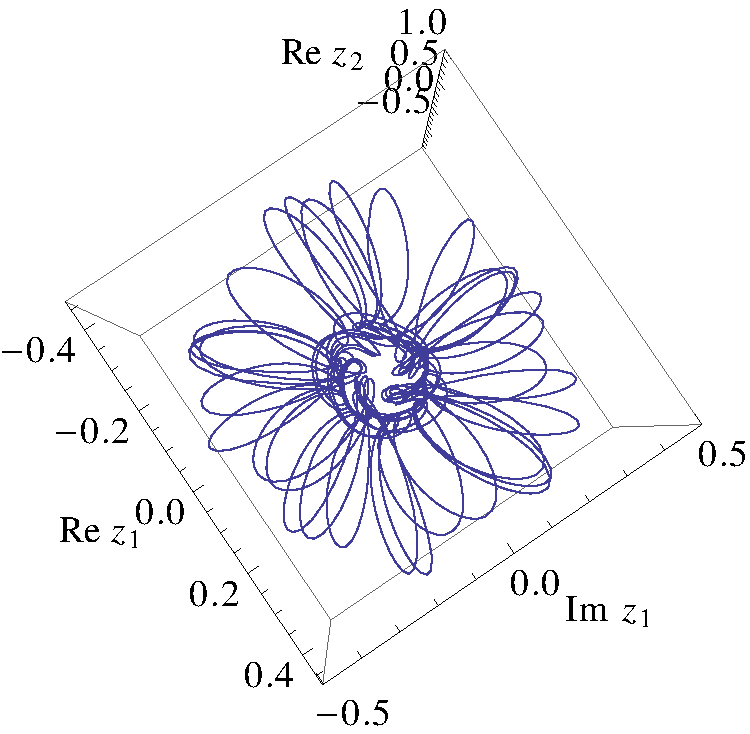
\includegraphics[width=0.35\textwidth]{dangelmayrZ}~
 (b) 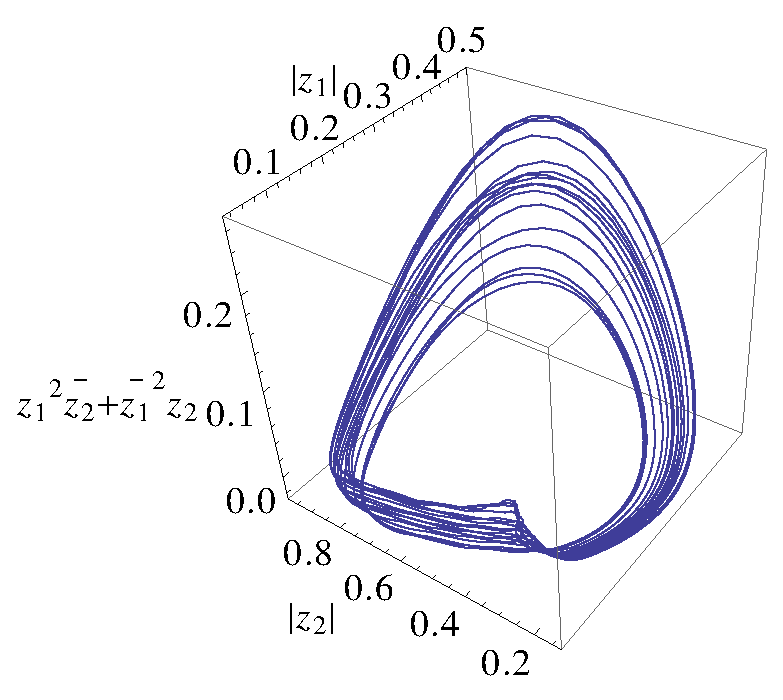
\includegraphics[width=0.35\textwidth]{dangelmayrAGH}~
\caption{Projections of Dangelmayr system \refeq{eq:DangSO2}
``attractor'' for $\mu_1 = -0.337,\, \mu_2 = 0.27,\, c_1 = 1,\, c_2 =
-1,\, a_1 = -1.5,\, a_2 = -6.19,\, b_1 = 1.583,\,  b_2 = -0.115,\, e_2 =
1.211$
(a) in equivariant \statesp\ coordinates
    $\{x_1, y_1 ,x_2, y_2\}$
    % $\Re z_1,\,\Im z_1,\,\Re z_2$.
(b) in invariant coordinates
    $\{\sqrt{u}, \sqrt{v}, w\}$
% used by Armbruster \etal\rf{AGHO288}
% $|z_1|,\, |z_2|,\, z_1^2 \bar{z}_2 + \bar{z}_1^2 z_2$.
}
 \label{fig:dangelmayrChaos}
\end{figure}
%%%%%%%%%%%%%%%%%%%%%%%%%%%%%%%%%%%%%%%%%%%%%%%%%%%%%%%%%%%%%%%%%%%%%%%%%%%%%%%%%%%%%

\item[2012-04-21 Evangelos]
The Dangelmayr system\rf{Dang86} written in complex coordinates $z_1,z_2$
is given in \refeq{eq:DangSO2} I have replaced symmetry breaking term $e$
here and in \refeq{eq:AGpolar} with $e_2$ since in this constant is
naturally paired with $\mu_2$. See also Armbruster, Guckenheimer and
Holmes\rf{AGHO288} flow with $\On{2}$ symmetry, here \refeq{eq:AGH}. In
\texttt{siminos/cgang/Evangelos/dangelmayr\_so2\_int.nb} I integrate
\refeq{eq:DangSO2} rather than the polar form \refeq{eq:AGpolar}, as the
former has no dangerous denominators.

\item[2012-04-25 Evangelos] Yet another snapshot of {\twoMode}
system with Predrag's modification, for different parameters. This looks
like an attractor made of two pieces, so it might be complicated enough
to demonstrate slicing. However I have yet no insight on whether there
are really two distinct topological mechanisms hidden here and what
controls them. Once relative equilibria are located, we should add them
here. The parameters are
\[
 \mu_1 = -0.337,\, \mu_2 = 0.27,\, c_1 = 1,\, c_2 = 1,\,
 a_1 = -0.4,\, a_2 = -6,\, b_1 = 1.6,\,  b_2 = -0.1,\, e_2 = 1.217
 \,.
\]

%%%%%%%%%%%%%%%%%%%%%%%%%%%%%%%%%%%%%%%%%%%%%%%%%%%%%%%%%%%%%%%%%%%%
 \begin{figure}[h]
%% ES created with siminos/cgang/Evangelos/dangelmayr_so2_plot.nb
\centering
 (a) 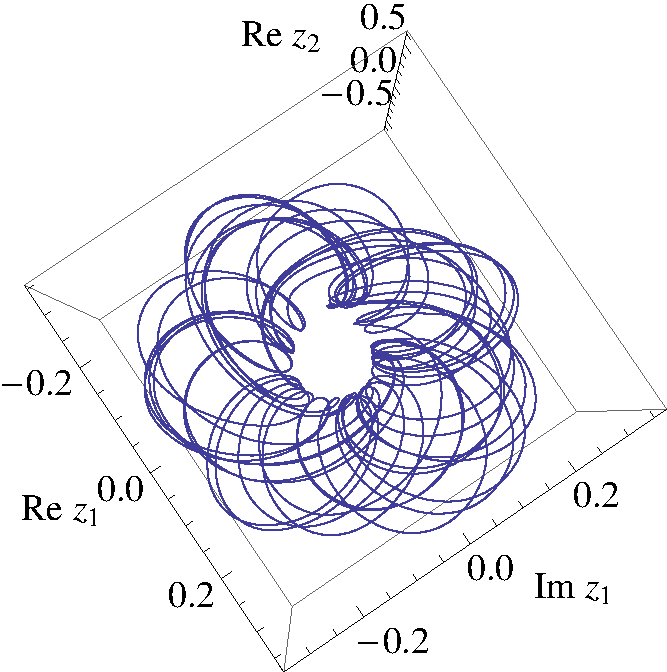
\includegraphics[width=0.35\textwidth]{dangelmayrZ2}~
 (b) 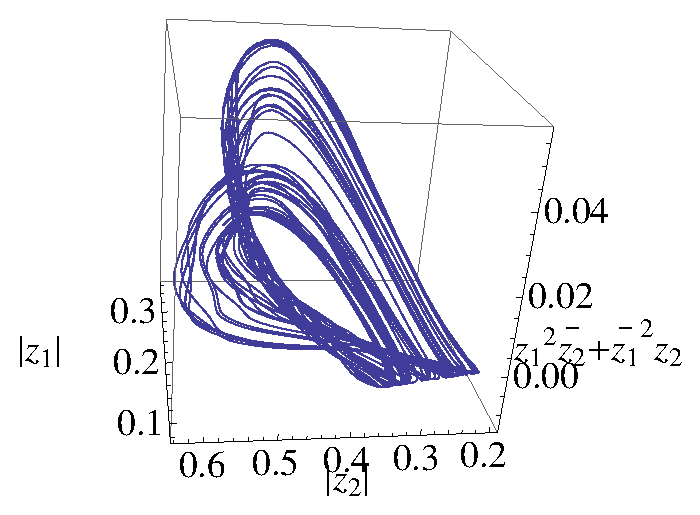
\includegraphics[width=0.35\textwidth]{dangelmayrAGH2}~
\caption{Projections of Dangelmayr system \refeq{eq:DangSO2}
``attractor'' for $\mu_1 = -0.337,\, \mu_2 = 0.27,\, c_1 = 1,\, c_2 = 1,\,
a_1 = -0.4,\, a_2 = -6,\, b_1 = 1.6,\,  b_2 = -0.1,\, e_2 = 1.217\,.$
(a) in original state space variables $\Re z_1,\,\Im z_1,\,\Re z_2$.
(b) in invariant coordinates used by
Armbruster \etal\rf{AGHO288}
$|z_1|,\, |z_2|,\, z_1^2 \bar{z}_2 + \bar{z}_1^2 z_2$.
}
 \label{fig:dangelmayrChaos2}
\end{figure}
%%%%%%%%%%%%%%%%%%%%%%%%%%%%%%%%%%%%%%%%%%%%%%%%%%%%%%%%%%%%%%%%%

\item[2012-04-27 Predrag] \refFig{fig:dangelmayrChaos2}\,(b) is one of 4
projections from the 4\dmn\ invariant polynomials $\{u,v,w,q\}$ dynamics
on any three of them. I would prefer that all such projections are linear
in coordinates (otherwise small $z_i$ really get scrunched), so please
plot $\{|u|^{1/2},|v|^{1/2},w/u |v|^{1/2} ,q/u |v|^{1/2} \}
= \{r_1,r_2, \cos\psi, \sin\psi \}$, or similar...


\item[2012-04-29 Predrag to Daniel]
% Thanks for fixing the pesky factor of 2 as well.
To summarize: \twoMode\ \reqva\ are the zeros of:
\bea
\tilde{f}(\tilde{u},\tilde{v}) &=&
  \tilde{u}\,A_1 - \tilde{v}\,A_2 = 0
\,,\qquad\qquad\qquad  deg(\tilde{f}) = 2
\continue
\tilde{g}(\tilde{u},\tilde{v}) &=&
 \left(A_1^2
 - c_1\,\tilde{v}\right)
 \left(\tilde{u}+2\,\tilde{v}\right)^2
 +e_2^2\,\tilde{v}^2 = 0
\,,\qquad  deg(\tilde{g}) = 4
\continue
 && \mbox{where }
A_1 = \mu_1+\tilde{a_1}\,\tilde{u}+\tilde{b_1}\,\tilde{v}
\,,\quad
A_2 = \mu_2+\tilde{a_2}\,\tilde{u}+\tilde{b_2}\,\tilde{v}
\,,
\nnu %\label{PKinvEqs5a}
\eea
in the positive $\tilde{u},\tilde{v} > 0$ quadrant (see
\refeq{PKinvEqs5a} for details). $g(u,v)$ and especially $f(u,v)$ look
pretty simple, so I'm thinking one can simply color-code their signs
(zeros are then 'nodal lines'). The \reqva\ are the intersections of two
sets of curves - might be a quick way to develop an intuition about roles
of various parameters, especially if you code it as something interactive
where parameters are sliders.

\item[2012-04-30 Predrag to C Gang] Evangelos
\texttt{Evangelos/dangelmayr\_so2\_int.nb} is a really cute toy - try it!

\item[2012-04-30 Predrag to Evangelos] I suggest using the 8 (or 7)
parameters of the rescaled \refeq{PKinvEqs5a} (hope I introduced no
further errors), and showing the value of a parameter under its slider
(at least, I cannot see it). There will be a bunch of constraints on the
parameters, Daniel and I will list them in as we find them.

\item[2012-04-30 Evangelos to Predrag] You can see the value of a parameter by
clicking on the cross next to the slidebar. I'll see if I can make it appear
permanently. I switched to unscaled variables while debugging the code but
I'm thinking not to switch back. The reason is that $c_1$ and $c_2$ in
Dangelmayr's paper can only take the values $\pm1$ and I follow this in
\texttt{dangelmayr\_so2\_int.nb}, so the gain in search space reduction is
not huge compared to the potential errors if I use 2 sets of parameters.
Also it keeps the code more readable. If we relax
restrictions on $c_1$, $c_2$, I will certainly switch to scaled variables.

\item[2012-05-02 Evangelos to Predrag] Now parameter values appear  bellow
sliders by default (thanks to local Mathematica expert Achilleas Lazarides).

\item[2012-04-30 Evangelos] In \texttt{siminos/cgang/Evangelos/dangelmayr\_so2\_int.nb}
I plot nullclines of \refeq{PKinvEqs5} to help with counting the number of
zeros. You can use some slidebars to vary parameters and experiment. You can
also experiment with phase-space plots of a typical trajectory and any relative
equilibria found numerically.

\item[2012-04-30 Evangelos] In \texttt{dangelmayr\_so2\_int.nb}, apart from
the nullclines, I plot the zero contour of $w^2+q^2-4u^2v$ to check whether
the syzygy is satisfied. It appears that the latter coincides with the $g(u,v)=0$
contour. Where does this come from? In deriving $f(u,v)=g(u,v)=0$ we did not
use the syzygy (at least not when I rederived it), so I thought it would impose
a further constraint satisfied exactly at the intersection of $f(u,v)=0$,
$g(u,v)=0$ for valid solutions. Why does it instead coincide with $g(u,v)$?

\item[2012-04-30 Evangelos to Predrag] I've tried your $\mu_1>-\mu_2>0$
suggestion but I cannot detect an interesting case. On the other hand with
$\mu_2>-\mu_1>0$ I find chaos but no relative equilibria. We need to get more
insight into stability of relative equilibria.


\item[2012-05-04 Sarah]
\HREF{http://www.snippyhaines.net/demos/cdf_index.htm}{Here's a first
stab} at an interactive R\"ossler web page.  It works on IE, but only
somewhat on Firefox.

\item[2012-05-06  Predrag to Sarah]
You might want to try to turn \texttt{Evangelos/dangelmayr\_so2\_int.nb}
into a {\twoMode} Wolfram CDF demonstration - it has sliders for various
parameters, and it should just work off the bat. We still have to settle
on a good example of chaos that requires two templates.

\item[2012-07-30 Evangelos] In \texttt{Evangelos/dangelmayr\_so2\_int.nb} I now color-code the $(u-v)$-plane according
to the sign of \refeq{2ModeStabTraceES} when plotting the zero-contours of $f(u,v)$ and $g(u,v)$ to help in detecting
a parameter region with two hyperbolic relative equilibria. 

\item[2012-07-30 Evangelos] I've allowed for $e_1 \neq 0$ in  \texttt{Evangelos/dangelmayr\_so2\_int.nb}, in order to
allow for a second ``frequency'' in the system, maybe generating richer dynamics. Have not played with it yet. Expressions used
to locate (relative) equilibria need to be modified accordingly.


\item[2012-05-07  Predrag to Chaos Gang] It's not over until it is over.



Time to go to bed...
\end{description}
